\documentclass[9pt, spanish]{entcs}
\usepackage{entcsmacro}

% Spanish accents
\usepackage[spanish]{babel}
\selectlanguage{spanish}
\usepackage[utf8]{inputenc}


% The mathtools package
% http://texdoc.net/texmf-dist/doc/latex/mathtools/mathtools.pdf
% https://www.codecogs.com/latex/eqneditor.php
\usepackage{mathtools}

% Algorithmic package
\usepackage{algpseudocode}
\usepackage{algorithm}
%\usepackage{algorithmic}
\usepackage{listings}

% Positioning of Figures H
\usepackage{float}

% Glossary of terms
\usepackage{glossaries}
\makeglossaries
% https://www.overleaf.com/learn/latex/Glossaries

\newacronym{AFD}{AFD}{\textit{Autómata Finito Determinista}}

\newglossaryentry{endpoints}
{
	name=puntos finales,
	description={Dos vértices conectados por una arista}
}

\newglossaryentry{symbol}
{
	name=símbolo,
	description={Un dato arbitrario que tiene algún significado o efecto en la máquina. A estos símbolos también se les llama "letras" o "átomos"}
}

\newglossaryentry{string}
{
	name=cadena,
	description={Una cadena finita formada por la concatenación de un número de símbolos}
}

\newglossaryentry{substring}
{
	name=subcadena,
	description={Una subcadena (segmento, subpalabra o factor) de una cadena es cualquier secuencia de símbolos consecutivos que aparecen en la cadena. En lenguaje formal, $t$ es una subcadena de $S$ sí y sólo si existe $x, y \in \Sigma^\ast$ tal que $S = xty$
	}
}

\newglossaryentry{prefix}
{
	name=prefijo,
	description={Un prefijo es una subcadena que aparece al principio de una cadena. Formalmente, $t$ es un prefijo de $S$ sí y sólo hay algún $y \in \Sigma^\ast$ tal que $S = ty$}
}

\newglossaryentry{suffix}
{
	name=sufijo,
	description={Un sufijo es una subcadena que aparece al final de una cadena. Formalmente, $t$ es un sufijo de $S$ sí y sólo hay algún $x \in \Sigma^\ast$ tal que $S = xt$}
}

% http://www.m-hikari.com/ams/ams-2014/ams-125-128-2014/singhAMS125-128-2014.pdf

\newglossaryentry{alphabet}
{
	name=alfabeto,
	description={Conjunto finito de símbolos. Un alfabeto se indica normalmente con $\Sigma$, que es el conjunto de letras en un alfabeto}
}

\newglossaryentry{language}
{
	name=lenguaje,
	description={Un conjunto de palabras, formado por símbolos en un alfabeto dado. Puede ser infinito}
}

% Clausura de Kleene

\begin{document}
	\begin{frontmatter}
	\title{Suffix Automaton} 
	\author{Andrés Valencia Oliveros\thanksref{myGitHub}\thanksref{myEmail}}
	\address{Facultad de Ingeniería, Diseño e Innovación\\ 
		Institución Universitaria Politécnico Grancolombiano\\
		Bogotá, Colombia
	}
	\thanks[myGitHub]{GitHub: 
		\href{https://github.com/anvalenciao/SuffixAutomaton}{\texttt{anvalenciao}}
	}
	\thanks[myEmail]{Email: 
		\href{mailto:anvalenciao@poligran.edu.co}{
			\texttt{\normalshape anvalenciao@poligran.edu.co}
		}
	}

	\renewcommand{\abstractname}{\textbf{Resumen}}
	\begin{abstract}
		
	\end{abstract}

	\begin{keyword}
		
	\end{keyword}
\end{frontmatter}
	\section{Introducción}\label{intro}

	\section{Grafo dirigido}\label{DirectedGraph}
\subsection{Grafo dirigido o digrafo}
Un grafo \( G(V,E) \) es una colección de puntos, llamados vértices o nodos \( V = \{ v_1, v_2, \dots \} \), y segmentos de línea que conectan esos puntos, llamados aristas o arcos (en inglés \textit{edges}) \( E = \{ e_1, e_2, \dots \} \); cada arista \( e \) tiene dos \textit{\gls{endpoints}}, que son vértices.

Un digrafo o grafo dirigido \( G(V,E) \) se define de manera similar a un grafo, excepto que el par de \textit{\gls{endpoints}} \( (u, v) \) de cada arista ahora está ordenado. Se escribe \( u \xrightarrow{\text{e}} v \), dónde \( u \) es el vértice inicial de \( e \); y \( v \) es el vértice final de \( e \). Se dice que la arista \( e \) está dirigida de \( u \) a \( v \) \cite{book:even2011graph}.

\begin{figure}[H]
	\centering
	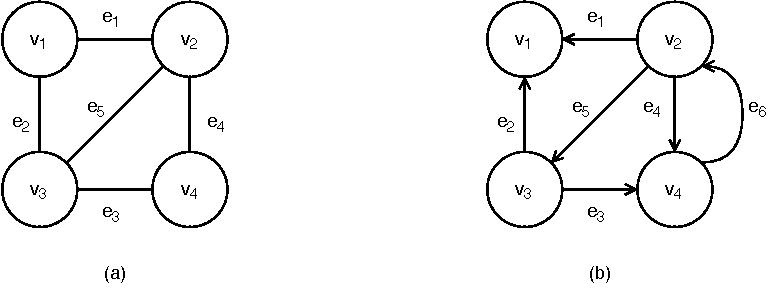
\includegraphics[width=0.8\linewidth]{doc/DirectedGraph/img/directed-undirected-graph}
	\caption{Tipos de grafos. (a) No dirigido. (b) Dirigido o digrafo. }
	\label{fig:directed-undirected-graph}
\end{figure}
	\section{Autómata finito determinista}\label{FiniteAutomaton}
Formalmente, un autómata finito es una 5-tupla ($Q, \Sigma, q_{0}, \delta, F$) donde:

\begin{itemize}
	\item $Q$, es un conjunto finito de estados;
	\item $\Sigma$, es un conjunto finito de \glspl{symbol} llamado \gls{alphabet};
	\item $q_{0}\in Q$ es el estado inicial;
	\item $\delta \colon Q\times \Sigma \to Q$ es una función de transición;
	\item $F\subseteq Q$ es un conjunto de estados finales o de aceptación.
\end{itemize}

Un \acrfull{AFD}, es un autómata/máquina que tiene un número finito de estados y además es un sistema determinista, es decir, para cada \gls{symbol} de entrada, se puede determinar el estado al que se moverá el autómata \cite{wiki:Automata_finito}. 

Un \acrshort{AFD} está representado por un grafo dirigido llamado diagrama de estado.

\begin{itemize}
	\item Los estados son representados por vértices o nodos $Q = \{ S_1, S_2, S_3, \dots \}$.
	\item Las aristas o arcos etiquetados con un \gls{alphabet} $\Sigma$, representan las transiciones $\delta$.
	\item El estado inicial $q_{0}$ se denota por una sola arista entrante vacía.
	\item El o los estados finales $F$ están indicados por círculos dobles.
	\item Cada transición se escribe  $\delta ( q_1, \sigma ) = q_2$,  también se puede denotar como $q_1 \xrightarrow{\sigma} q_2$.
\end{itemize}

\begin{example}
	El siguiente ejemplo es de un \acrshort{AFD} $L$, con un alfabeto binario, que reconoce el lenguaje regular conformado exclusivamente por las cadenas con un número par de ceros y un número par de unos.
	
	$M = (Q, \Sigma, q_{0}, \delta, F)$ donde:
	\begin{itemize}
		\item $Q = \{S_1, S_2, S_3, S_4 \}$
		\item $\Sigma = \{ 0, 1 \}$
		\item $q_0 = S_1$
		\item $F = \{ S1 \}$
		\item $\delta:  
				\delta(S_1, 0) = S_3, 
				\delta(S_1, 1) = S_2,
				\delta(S_2, 0) = S_4,
				\delta(S_2, 1) = S_1,
				\delta(S_3, 0) = S_1,
				\delta(S_3, 1) = S_4,
				\delta(S_4, 0) = S_2,
				\delta(S_4, 1) = S_3
			$
	\end{itemize}
	
	\begin{figure}[H]
		\centering
		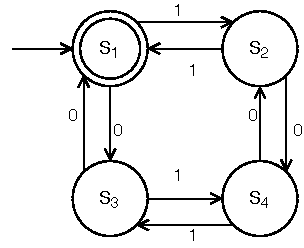
\includegraphics[width=0.4\linewidth]{doc/FiniteAutomaton/img/AFD}
		\caption{El diagrama de estado de $L$}
		\label{fig:AFD}
	\end{figure}
	
	El lenguaje reconocido por $L$ es el lenguaje regular dado por la expresión regular \cite{stackoverflow:Biegeleisen2015}: 
	$$
	^\wedge(00|11|(01|10)(00|11)^\ast(01|10))^\ast \$
	$$
	
	La Figura \ref{fig:AFD} da un ejemplo de un autómata simple $M$ que acepta la cadena:
	$$
	1001101011001010010001
	$$

\end{example}

% https://en.wikipedia.org/wiki/Deterministic_finite_automaton
% https://es.wikipedia.org/wiki/Teor%C3%ADa_de_aut%C3%B3matas

	\section{Autómata de sufijo}\label{SuffixAutomaton}
Un autómata de sufijo es una estructura de datos eficiente y compacta, también conocido como Directed Acyclic Word Graph (DAWG), es el \acrshort{AFD} mínimo, que reconoce el conjunto de sufijos de una \gls{string} $S  = s_1 s_2 s_3 \dots s_n $ \cite{wiki:Suffix_automaton}, es decir, se puede usar un autómata sufijo para determinar si una \gls{string} $x$ es una \gls{substring} en tiempo lineal en su longitud $O(| x |)$ \cite{article:10.1016/j.tcs.2009.03.034}.


\gls{prefix}
\gls{suffix}

\subsection{Propiedades}

\subsubsection{Endpos}


% https://en.wikipedia.org/wiki/Suffix_automaton
% https://es.qaz.wiki/wiki/Suffix_automaton
% https://codeforces.com/blog/entry/20861
% https://static.googleusercontent.com/media/research.google.com/en//pubs/archive/35395.pdf
% https://stackoverflow.com/questions/24411000/what-is-a-suffix-automaton
% https://akshay.jaggi.co/blog/suffix-automata/
% https://saisumit.wordpress.com/2016/01/26/suffix-automaton/
% https://discuss.codechef.com/t/plant-editorial/45402
% https://cp-algorithms.com/string/suffix-automaton.html
% https://onlinejudge.org/index.php?option=onlinejudge&page=show_problem&problem=660
% https://sites.google.com/site/indy256/algo/suffix_automaton
% http://kiritow.com:3000/Kiritow/OJ-Problems-Source/src/e11349a42b5ca8a65621ba9cff78315deb482c15/.ACM-Templates/Data-Structures/suffix-automaton/main.cpp
% https://github.com/sourabh2311/Competitive-Programming/blob/master/SPOJ_NSUBSTR.cpp
% https://github.com/sourabh2311/Competitive-Programming/blob/master/UVA_719.cpp
% https://www.youtube.com/watch?v=axlgMCq7yTg&ab_channel=HowardCheng
% https://www.udebug.com/UVa/719
% https://www.wjyyy.top/1732.html

	\section{Algoritmo}\label{Algorithm}
% autómata finito determinista

	\printglossary[title=Glosario de términos, toctitle=Lista de términos]
	\renewcommand{\refname}{Referencias}
\bibliographystyle{ieeetr}
\bibliography{doc/Bibliography/articles,doc/Bibliography/proceedings,doc/Bibliography/books,doc/Bibliography/misc}
\end{document}